\documentclass{standalone}
\usepackage{tikz}
\usetikzlibrary{patterns, positioning}

\begin{document}
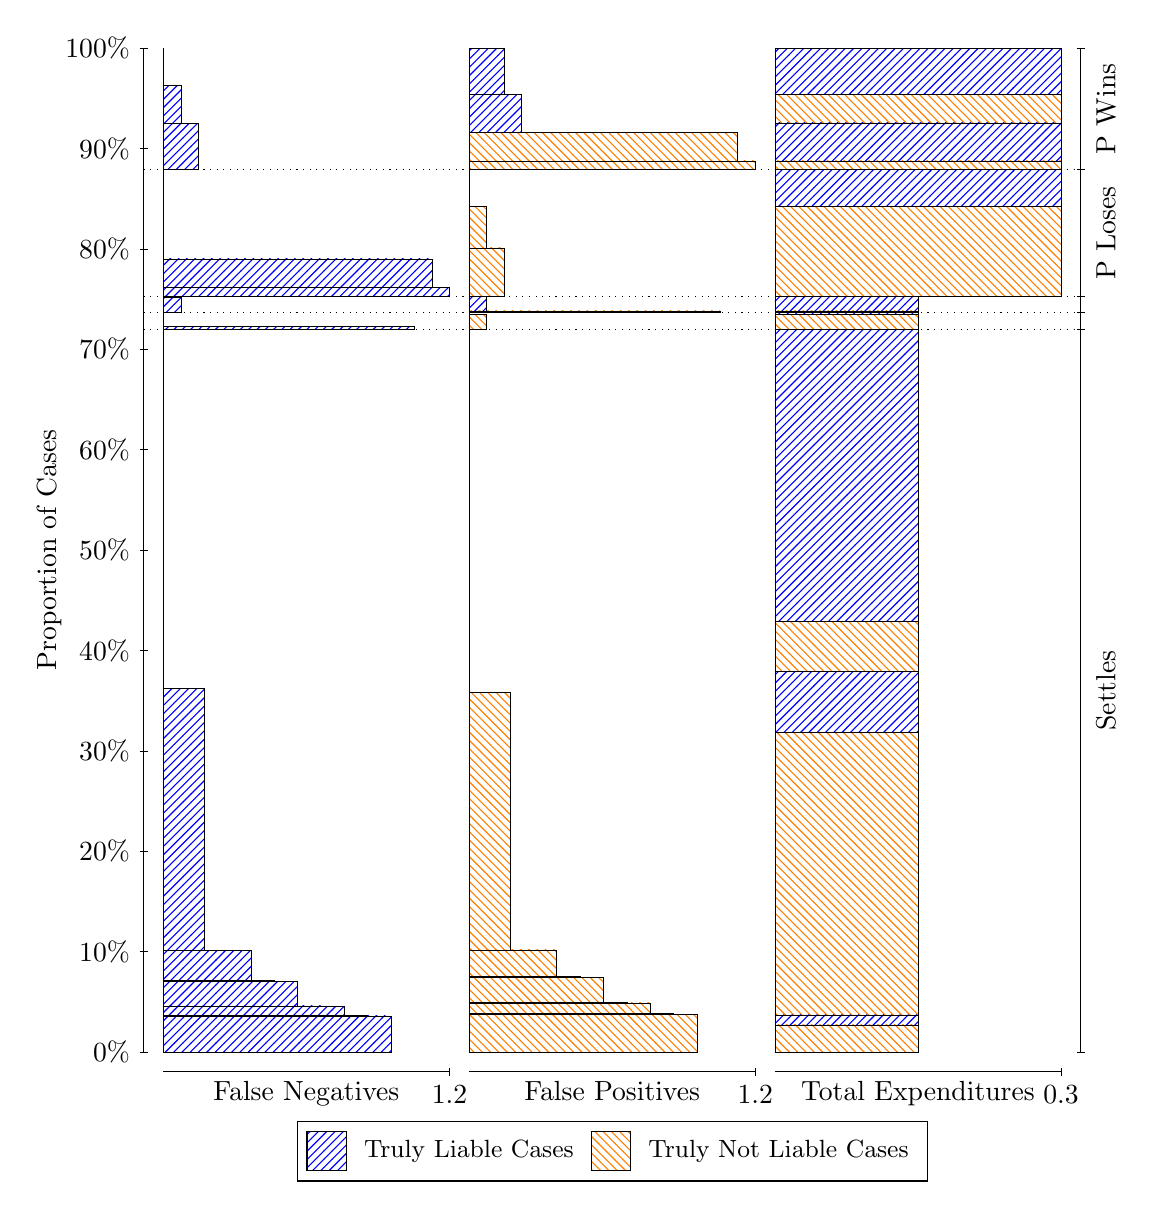
\begin{tikzpicture}
\draw[black, very thin] (1.5,1.75) -- (1.5,14.5);
\node[rotate=90, anchor=center] at (0.3, 8.125) {Proportion of Cases};
\draw[black, very thin] (1.45,1.75) -- (1.55,1.75);
\node[anchor=east] at (1.45, 1.75) {0\%};
\draw[black, very thin] (1.45,3.025) -- (1.55,3.025);
\node[anchor=east] at (1.45, 3.025) {10\%};
\draw[black, very thin] (1.45,4.3) -- (1.55,4.3);
\node[anchor=east] at (1.45, 4.3) {20\%};
\draw[black, very thin] (1.45,5.575) -- (1.55,5.575);
\node[anchor=east] at (1.45, 5.575) {30\%};
\draw[black, very thin] (1.45,6.85) -- (1.55,6.85);
\node[anchor=east] at (1.45, 6.85) {40\%};
\draw[black, very thin] (1.45,8.125) -- (1.55,8.125);
\node[anchor=east] at (1.45, 8.125) {50\%};
\draw[black, very thin] (1.45,9.4) -- (1.55,9.4);
\node[anchor=east] at (1.45, 9.4) {60\%};
\draw[black, very thin] (1.45,10.675) -- (1.55,10.675);
\node[anchor=east] at (1.45, 10.675) {70\%};
\draw[black, very thin] (1.45,11.95) -- (1.55,11.95);
\node[anchor=east] at (1.45, 11.95) {80\%};
\draw[black, very thin] (1.45,13.225) -- (1.55,13.225);
\node[anchor=east] at (1.45, 13.225) {90\%};
\draw[black, very thin] (1.45,14.5) -- (1.55,14.5);
\node[anchor=east] at (1.45, 14.5) {100\%};

\draw[black, very thin] (13.4,1.75) -- (13.4,14.5);
\draw[black, very thin] (13.35,1.75) -- (13.45,1.75);
\node[anchor=west] at (13.35, 1.75) {};
\draw[black, very thin] (13.35,10.93) -- (13.45,10.93);
\node[anchor=west] at (13.35, 10.93) {};
\draw[black, very thin] (13.35,11.144) -- (13.45,11.144);
\node[anchor=west] at (13.35, 11.144) {};
\draw[black, very thin] (13.35,11.348) -- (13.45,11.348);
\node[anchor=west] at (13.35, 11.348) {};
\draw[black, very thin] (13.35,12.957) -- (13.45,12.957);
\node[anchor=west] at (13.35, 12.957) {};
\draw[black, very thin] (13.35,14.5) -- (13.45,14.5);
\node[anchor=west] at (13.35, 14.5) {};

\draw[black, very thin, pattern color=blue, pattern=north east lines] (1.75,1.75) rectangle (4.6418,2.2093);
\draw[black, very thin, pattern color=blue, pattern=north east lines] (1.75,2.2093) rectangle (4.3452,2.2115);
\draw[black, very thin, pattern color=blue, pattern=north east lines] (1.75,2.2115) rectangle (4.0486,2.3297);
\draw[black, very thin, pattern color=blue, pattern=north east lines] (1.75,2.3297) rectangle (3.752,2.3353);
\draw[black, very thin, pattern color=blue, pattern=north east lines] (1.75,2.3353) rectangle (3.4554,2.6503);
\draw[black, very thin, pattern color=blue, pattern=north east lines] (1.75,2.6503) rectangle (3.1588,2.662);
\draw[black, very thin, pattern color=blue, pattern=north east lines] (1.75,2.662) rectangle (2.8622,3.0366);
\draw[black, very thin, pattern color=blue, pattern=north east lines] (1.75,3.0366) rectangle (2.5656,3.0426);
\draw[black, very thin, pattern color=blue, pattern=north east lines] (1.75,3.0426) rectangle (2.269,6.3641);
\draw[black, very thin, pattern color=orange, pattern=north west lines] (1.75,6.3641) rectangle (1.75,10.93);
\draw[black, very thin, pattern color=blue, pattern=north east lines] (1.75,10.93) rectangle (4.9384,10.961);
\draw[black, very thin, pattern color=orange, pattern=north west lines] (1.75,10.961) rectangle (1.75,11.144);
\draw[black, very thin, pattern color=blue, pattern=north east lines] (1.75,11.144) rectangle (1.9724,11.33);
\draw[black, very thin, pattern color=orange, pattern=north west lines] (1.75,11.33) rectangle (1.75,11.348);
\draw[black, very thin, pattern color=blue, pattern=north east lines] (1.75,11.348) rectangle (5.3833,11.461);
\draw[black, very thin, pattern color=blue, pattern=north east lines] (1.75,11.461) rectangle (5.1609,11.821);
\draw[black, very thin, pattern color=orange, pattern=north west lines] (1.75,11.821) rectangle (1.75,12.957);
\draw[black, very thin, pattern color=blue, pattern=north east lines] (1.75,12.957) rectangle (2.1949,13.546);
\draw[black, very thin, pattern color=blue, pattern=north east lines] (1.75,13.546) rectangle (1.9724,14.028);
\draw[black, very thin, pattern color=orange, pattern=north west lines] (1.75,14.028) rectangle (1.75,14.5);
\draw[black, very thin, pattern color=orange, pattern=north west lines] (5.6333,1.75) rectangle (8.5252,2.2295);
\draw[black, very thin, pattern color=orange, pattern=north west lines] (5.6333,2.2295) rectangle (8.2286,2.2353);
\draw[black, very thin, pattern color=orange, pattern=north west lines] (5.6333,2.2353) rectangle (7.932,2.3735);
\draw[black, very thin, pattern color=orange, pattern=north west lines] (5.6333,2.3735) rectangle (7.6354,2.3805);
\draw[black, very thin, pattern color=orange, pattern=north west lines] (5.6333,2.3805) rectangle (7.3388,2.7018);
\draw[black, very thin, pattern color=orange, pattern=north west lines] (5.6333,2.7018) rectangle (7.0422,2.7104);
\draw[black, very thin, pattern color=orange, pattern=north west lines] (5.6333,2.7104) rectangle (7.0422,2.7116);
\draw[black, very thin, pattern color=orange, pattern=north west lines] (5.6333,2.7116) rectangle (6.7456,3.0453);
\draw[black, very thin, pattern color=orange, pattern=north west lines] (5.6333,3.0453) rectangle (6.449,3.0465);
\draw[black, very thin, pattern color=orange, pattern=north west lines] (5.6333,3.0465) rectangle (6.1524,6.3157);
\draw[black, very thin, pattern color=blue, pattern=north east lines] (5.6333,6.3157) rectangle (5.6333,10.93);
\draw[black, very thin, pattern color=orange, pattern=north west lines] (5.6333,10.93) rectangle (5.8558,11.113);
\draw[black, very thin, pattern color=blue, pattern=north east lines] (5.6333,11.113) rectangle (5.6333,11.144);
\draw[black, very thin, pattern color=orange, pattern=north west lines] (5.6333,11.144) rectangle (8.8218,11.162);
\draw[black, very thin, pattern color=blue, pattern=north east lines] (5.6333,11.162) rectangle (5.8558,11.348);
\draw[black, very thin, pattern color=orange, pattern=north west lines] (5.6333,11.348) rectangle (6.0782,11.963);
\draw[black, very thin, pattern color=orange, pattern=north west lines] (5.6333,11.963) rectangle (5.8558,12.484);
\draw[black, very thin, pattern color=blue, pattern=north east lines] (5.6333,12.484) rectangle (5.6333,12.957);
\draw[black, very thin, pattern color=orange, pattern=north west lines] (5.6333,12.957) rectangle (9.2667,13.066);
\draw[black, very thin, pattern color=orange, pattern=north west lines] (5.6333,13.066) rectangle (9.0442,13.429);
\draw[black, very thin, pattern color=blue, pattern=north east lines] (5.6333,13.429) rectangle (6.3007,13.911);
\draw[black, very thin, pattern color=blue, pattern=north east lines] (5.6333,13.911) rectangle (6.0782,14.5);
\draw[black, very thin, pattern color=orange, pattern=north west lines] (9.5167,1.75) rectangle (11.333,2.0946);
\draw[black, very thin, pattern color=blue, pattern=north east lines] (9.5167,2.0946) rectangle (11.333,2.2206);
\draw[black, very thin, pattern color=orange, pattern=north west lines] (9.5167,2.2206) rectangle (11.333,5.8112);
\draw[black, very thin, pattern color=blue, pattern=north east lines] (9.5167,5.8112) rectangle (11.333,6.5856);
\draw[black, very thin, pattern color=orange, pattern=north west lines] (9.5167,6.5856) rectangle (11.333,7.216);
\draw[black, very thin, pattern color=blue, pattern=north east lines] (9.5167,7.216) rectangle (11.333,10.93);
\draw[black, very thin, pattern color=orange, pattern=north west lines] (9.5167,10.93) rectangle (11.333,11.113);
\draw[black, very thin, pattern color=blue, pattern=north east lines] (9.5167,11.113) rectangle (11.333,11.144);
\draw[black, very thin, pattern color=orange, pattern=north west lines] (9.5167,11.144) rectangle (11.333,11.162);
\draw[black, very thin, pattern color=blue, pattern=north east lines] (9.5167,11.162) rectangle (11.333,11.348);
\draw[black, very thin, pattern color=orange, pattern=north west lines] (9.5167,11.348) rectangle (13.15,12.484);
\draw[black, very thin, pattern color=blue, pattern=north east lines] (9.5167,12.484) rectangle (13.15,12.957);
\draw[black, very thin, pattern color=orange, pattern=north west lines] (9.5167,12.957) rectangle (13.15,13.066);
\draw[black, very thin, pattern color=blue, pattern=north east lines] (9.5167,13.066) rectangle (13.15,13.548);
\draw[black, very thin, pattern color=orange, pattern=north west lines] (9.5167,13.548) rectangle (13.15,13.911);
\draw[black, very thin, pattern color=blue, pattern=north east lines] (9.5167,13.911) rectangle (13.15,14.5);
\draw[black, dotted] (1.5,10.93) -- (13.4,10.93);
\draw[black, dotted] (1.5,11.144) -- (13.4,11.144);
\draw[black, dotted] (1.5,11.348) -- (13.4,11.348);
\draw[black, dotted] (1.5,12.957) -- (13.4,12.957);
\draw[black, very thin] (1.75,1.5) -- (5.3833,1.5);
\node[anchor=north] at (3.5667, 1.5) {False Negatives};
\draw[black, very thin] (5.3833,1.45) -- (5.3833,1.55);
\node[anchor=north] at (5.3833, 1.45) {1.2};

\draw[black, very thin] (5.6333,1.5) -- (9.2667,1.5);
\node[anchor=north] at (7.45, 1.5) {False Positives};
\draw[black, very thin] (9.2667,1.45) -- (9.2667,1.55);
\node[anchor=north] at (9.2667, 1.45) {1.2};

\draw[black, very thin] (9.5167,1.5) -- (13.15,1.5);
\node[anchor=north] at (11.333, 1.5) {Total Expenditures};
\draw[black, very thin] (13.15,1.45) -- (13.15,1.55);
\node[anchor=north] at (13.15, 1.45) {0.3};

\node[black, centered, rotate=90] at (13.72, 6.3399) {Settles};


\node[black, centered, rotate=90] at (13.72, 12.152) {P Loses};
\node[black, centered, rotate=90] at (13.72, 13.728) {P Wins};

\draw (7.449999999999999,1.5) node[draw=none] (baseCoordinate) {};
\begin{scope}[align=center]
        \matrix[scale=0.5, draw=black, below=0.5cm of baseCoordinate, nodes={draw}, column sep=0.1cm]{
            \node[rectangle, draw, minimum width=0.5cm, minimum height=0.5cm, pattern=north east lines, pattern color=blue] {}; &
            \node[draw=none, font=\small] (B) {Truly Liable Cases}; &
            \node[rectangle, draw, minimum width=0.5cm, minimum height=0.5cm, pattern=north west lines, pattern color=orange] {}; &
            \node[draw=none, font=\small] (B) {Truly Not Liable Cases}; \\
            };
\end{scope}

\end{tikzpicture}
\end{document}